\section{Introduction}
\label{sec:introduction}

\subsection{Motivation}
\label{sec:motivation}

Most Linux distributions are either conservative remixes of existing systems or
highly opinionated tools for a specific niche. Neither describes this project.

The dominant desktop operating systems have a structural problem. Windows works
against its own users: forced updates, advertisements in the start menu, and
background telemetry (automatic reporting of usage data to the vendor) that
nobody enabled. macOS is polished but locks users into an ecosystem designed to
keep them paying and dependent. Every Linux distribution, however technically
excellent, has failed to make the jump to people who simply want to use a
computer without becoming a system administrator. The gap between ``technically
capable'' and ``actually usable'' has not closed in thirty years.

This project exists to close that gap. It is a Linux-based operating system
built from scratch with a different set of priorities: one that integrates a
system-wide knowledge graph, AI interfaces, and modern tooling not as features
bolted on top, but as foundational infrastructure. It takes a clear stance on
user sovereignty, European software independence, and not being annoying to use.
If an operating system is being built in 2025 anyway, there is no reason to
repeat patterns from 1995.

\subsection{Target Audience}
\label{sec:audience}

The primary audience is people switching from macOS or Windows who want a
genuinely good alternative: modern in appearance, functional out of the box,
and respectful of their autonomy. Consumer-first, not enterprise-first. The
macOS user tired of lock-in but unwilling to compromise on quality. The Windows
user whose computer feels like it belongs to Microsoft more than to them. They
do not want to configure. They want to arrive and work, and feel like the
operating system is actually theirs.

Business deployment is a future consideration. The architecture supports managed
environments and administrator policies. However, one line does not move:
an administrator can configure defaults and restrict software; an administrator
cannot surveil users or override their personal data ownership. Company needs
will never come at the expense of user rights.

\subsection{Design Principles}
\label{sec:principles}

The following principles govern every design decision in this project. They are
not aspirational marketing language; they are constraints that break ties and
override convenience.

\paragraph{For the user, not for the platform.}
No advertisements, no tracking, no dark patterns, no telemetry without explicit
consent. When a conflict arises between the user's interest and anything
else, the user wins. This applies to business deployments as well: admin
policies configure the environment, they do not strip users of their data or
autonomy.

\paragraph{Independence by default.}
No mandatory cloud accounts. No dependency on services that can be switched
off by a company in another jurisdiction. The system works fully offline,
self-hosted, and without phoning home. Cloud features are opt-in extensions,
not prerequisites. This is a technical commitment, not a marketing label.

\paragraph{The knowledge graph belongs to you.}
All system intelligence runs locally by default. The knowledge graph, AI
context, and activity history do not leave the machine without an explicit user
action. Cloud AI providers are opt-in, configured by the user, and can be
removed entirely.

\paragraph{Quality of life over feature count.}
Small things matter. A system that warns you when something is quietly invading
your privacy, that remembers what you were working on, that switches themes
system-wide in one action: these are not large features. They are the difference
between a system that feels alive and one that feels like infrastructure.
Thoughtful small features beat impressive large ones that nobody uses.

\paragraph{Out of the box, not out of patience.}
Everything works on first boot. No hunting for drivers, no configuring package
managers, no reading wiki pages to get audio working. The standard use case
requires zero setup. Advanced configuration is always available, never required.

\paragraph{Future-oriented, not hype-driven.}
New technology gets used when it makes sense, not because it is trending. AI
integration and the knowledge graph are here because they genuinely change what
a personal computer can do. If a system is being built from scratch, there is no
excuse for dragging along outdated patterns because everyone else does.

\paragraph{Good-looking is not optional.}
A poor interface is a barrier to entry. The system must look better than what
users are coming from, on first boot. Visual quality is not vanity; it is
respect for the user's time and trust.

\paragraph{Coherent, not cobbled together.}
Shared configuration standards, shared theming, shared interfaces across all
system components. Change the accent color once and it propagates everywhere.
No component that looks like it was designed in a different decade by a different
team.

\paragraph{Pragmatic, not ideological.}
No purity tests. The goal is a useful, trustworthy system. That said: no
advertisements, no tracking, no dark patterns. Not because of ideology, but
because that is bad product design.

\paragraph{Bridges, not walls.}
Where established standards and existing implementations exist, compatibility
bridges are built rather than replacements. Apps built for other Linux desktops
run here. Standard Linux tools and hardware interfaces are supported. Nothing is
deliberately broken for the sake of purity.

\paragraph{Transparent by default.}
The system can explain what it is doing and why, in plain language. Not buried
in logs, but surfaced where the user can see and act on it. A system legible to
its user is a system the user can trust.

\subsection{Positioning}
\label{sec:positioning}

Figure~\ref{fig:positioning} illustrates the design space this project occupies
relative to existing systems. The goal is the upper-right quadrant: high
usability \emph{and} high user sovereignty. This combination does not currently
exist in any mainstream desktop operating system.

\begin{figure}[htbp]
\centering
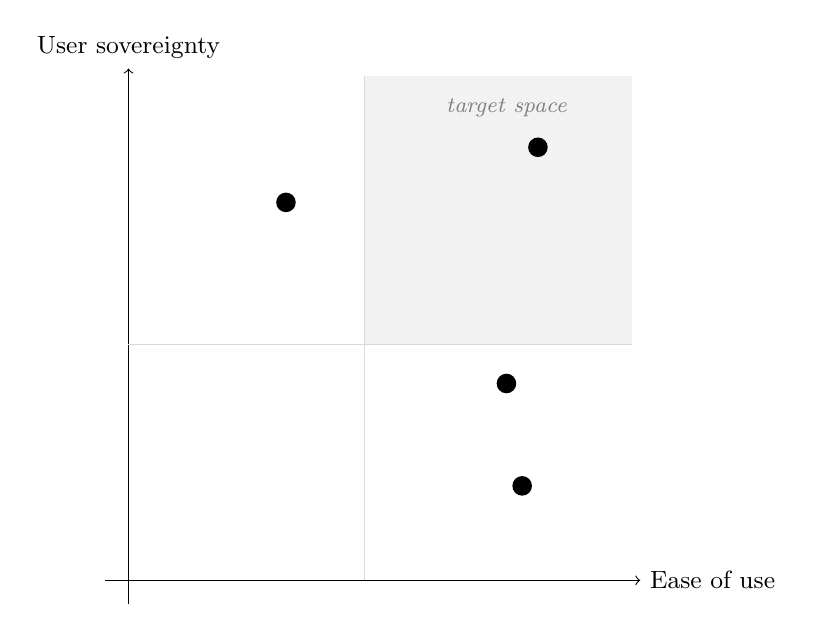
\begin{tikzpicture}[
  dot/.style={circle, fill, inner sep=2.5pt},
  label/.style={font=\small},
]
  % Axes
  \draw[->] (-0.3,0) -- (6.5,0) node[right, font=\small] {Ease of use};
  \draw[->] (0,-0.3) -- (0,6.5) node[above, font=\small] {User sovereignty};

  % Quadrant shading
  \fill[gray!10] (3,3) rectangle (6.4,6.4);

  % Gridlines
  \draw[gray!30] (3,0) -- (3,6.4);
  \draw[gray!30] (0,3) -- (6.4,3);

  % Existing systems
  \node[dot, label=below right:{Windows}]   at (5.0, 1.2) {};
  \node[dot, label=below right:{macOS}]     at (4.8, 2.5) {};
  \node[dot, label=above left:{\parbox{2.2cm}{\centering Typical\\[-2pt]Linux distro}}]
                                            at (2.0, 4.8) {};

  % This project
  \node[dot, fill=black, label=above right:{\textbf{[Project]}}]
                                            at (5.2, 5.5) {};

  % Quadrant label
  \node[gray, font=\footnotesize\itshape] at (4.8, 6.0) {target space};

\end{tikzpicture}
\caption{Design space: ease of use versus user sovereignty. Existing mainstream
systems occupy either the lower-right (usable but extractive) or upper-left
(sovereign but inaccessible) quadrants. This project targets the upper-right.}
\label{fig:positioning}
\end{figure}

\subsection{What This Project Is Not}
\label{sec:nongoals}

Clarifying what this project is not is as important as describing what it is.

It is not a minimal system stripped to its essentials. There is real complexity
here, and that is intentional: a system that works for non-technical users
requires more infrastructure, not less.

It is not a fully declarative system where every piece of software is managed
through configuration files. Reproducibility is a goal; mandatory declarative
configuration is not.

It is not a distro aimed at advanced Linux users only. New users are explicitly
part of the target. Advanced users are welcome and well-served, but they are not
the primary design constraint.

It is not a corporate product that happens to be open source. Business use is
secondary; user rights are not negotiable.

It is not a Windows or macOS clone. The goal is a better alternative, not a
familiar imitation.
